\section{Annexe}
  \subsection{Bibliographie}
    \begin{itemize}
    	\item "Apprendre à programmer avec Python 3" - Gérard Swinnen
    	\item \href{http://effbot.org/}{http://effbot.org/}
    \end{itemize}

  \subsection{Liste des Work Packages}
  \begin{figure}[h!]
    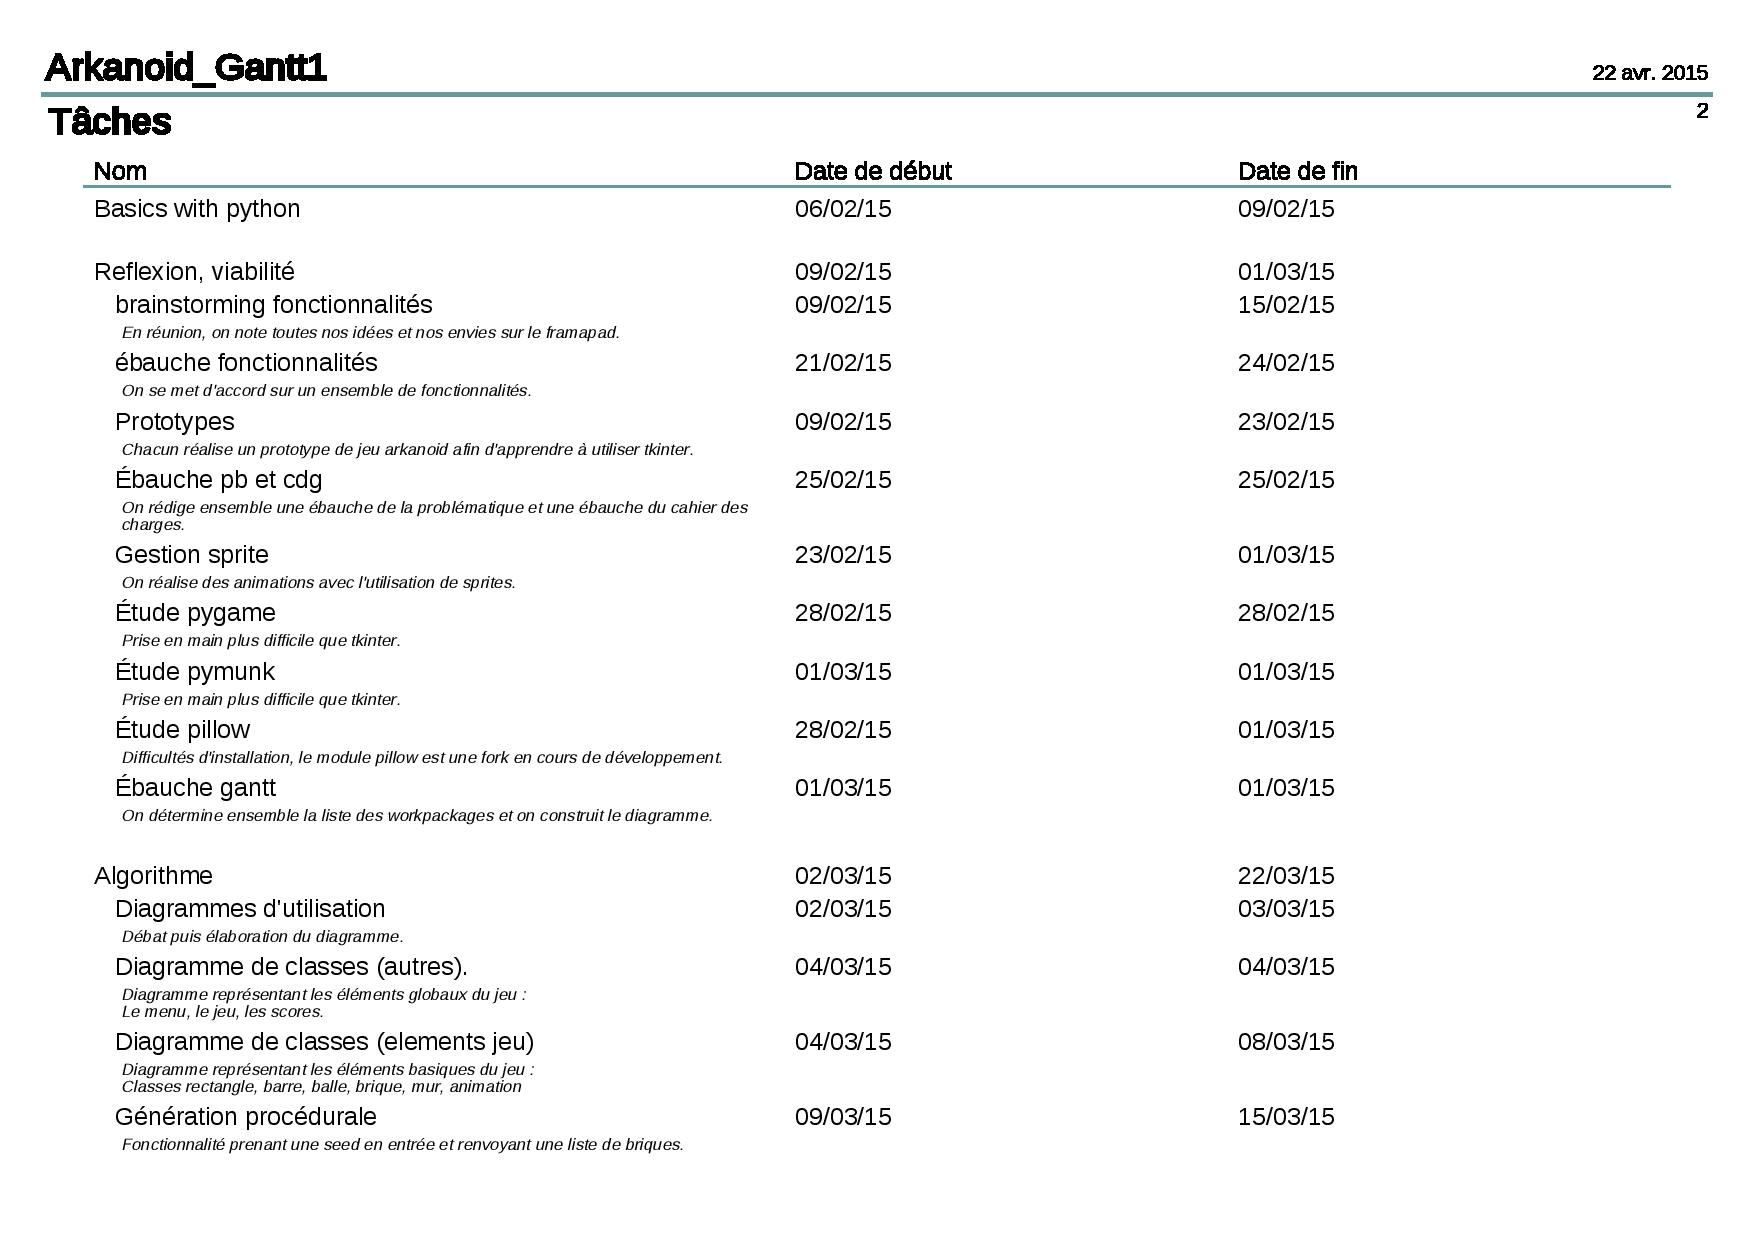
\includegraphics[width=1\textwidth]{img/WK1.jpg}\\
  \end{figure}
  \begin{figure}[h!]
    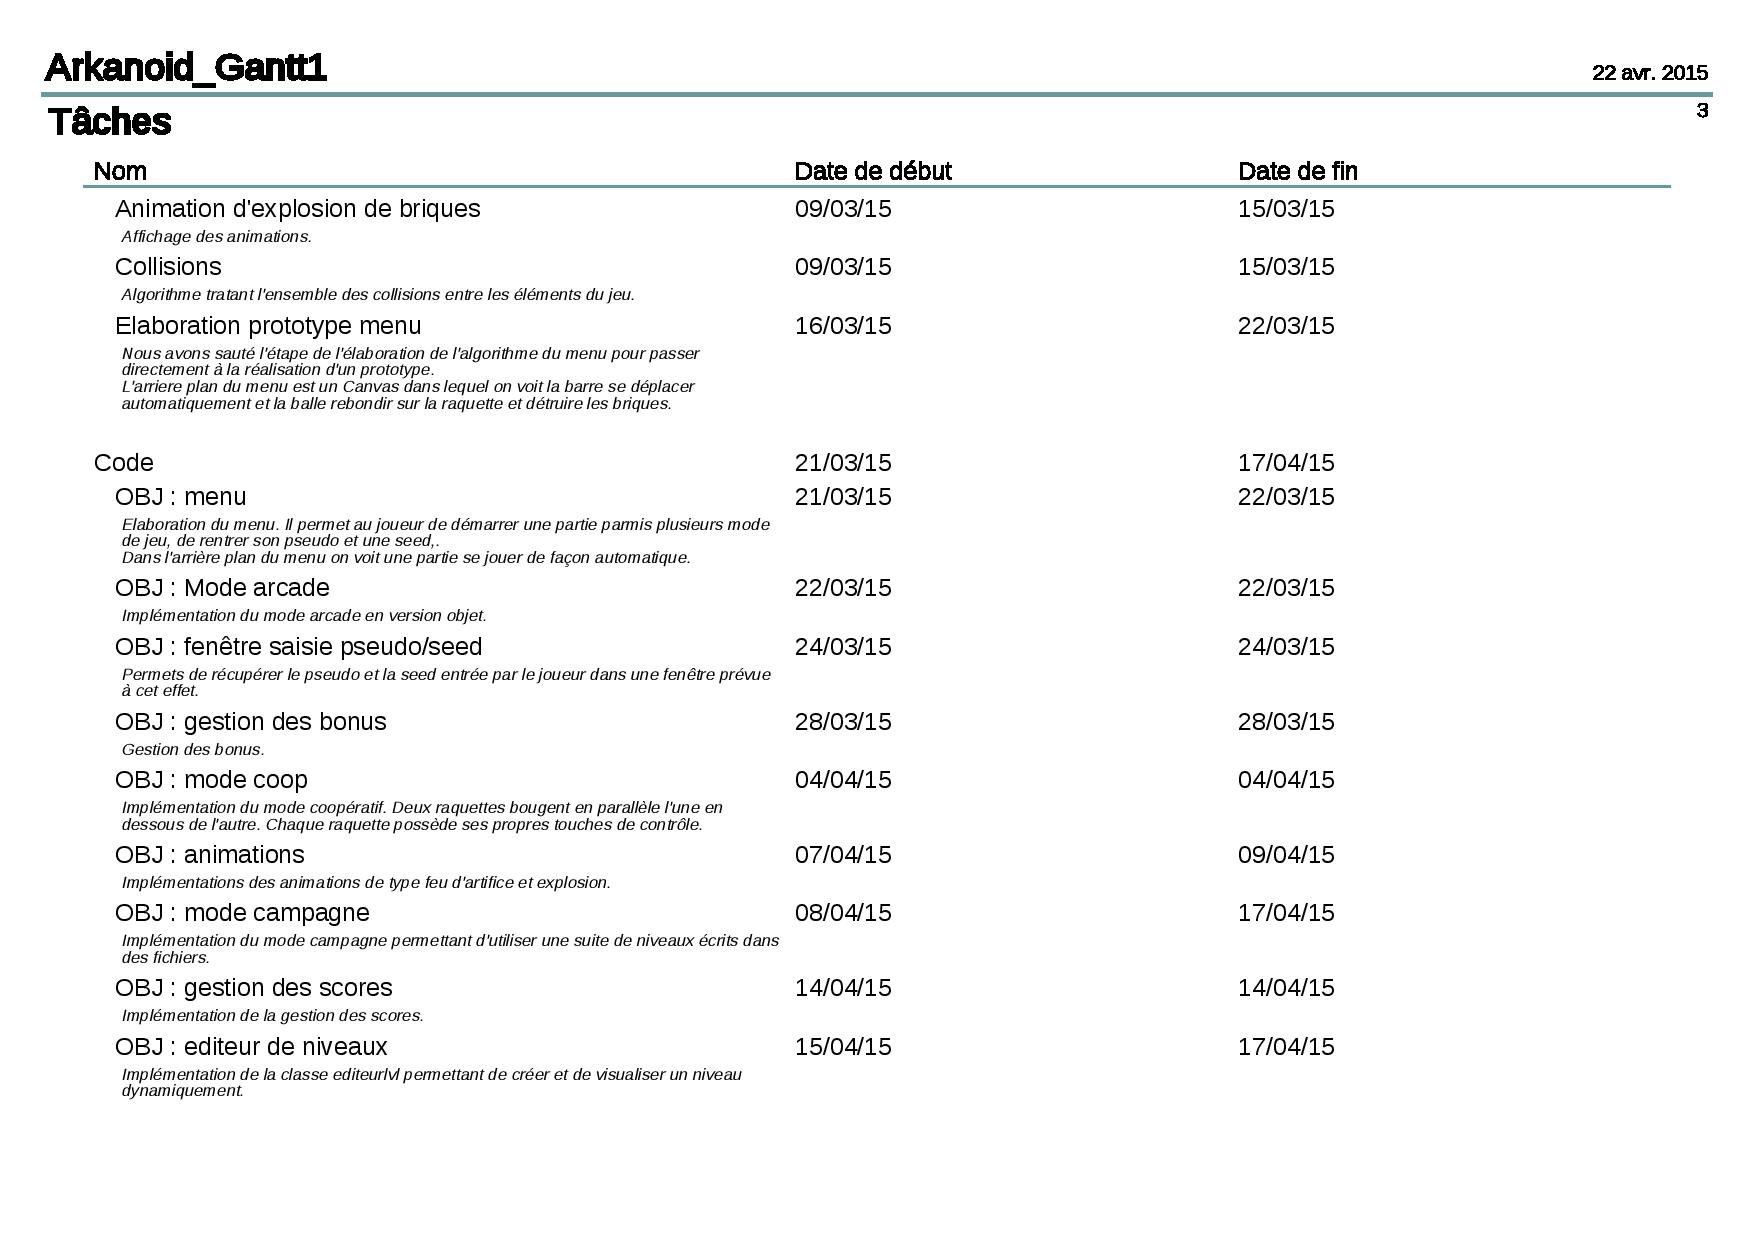
\includegraphics[width=1\textwidth]{img/WK2.jpg}\\
  \end{figure}
  \begin{figure}[h!]
    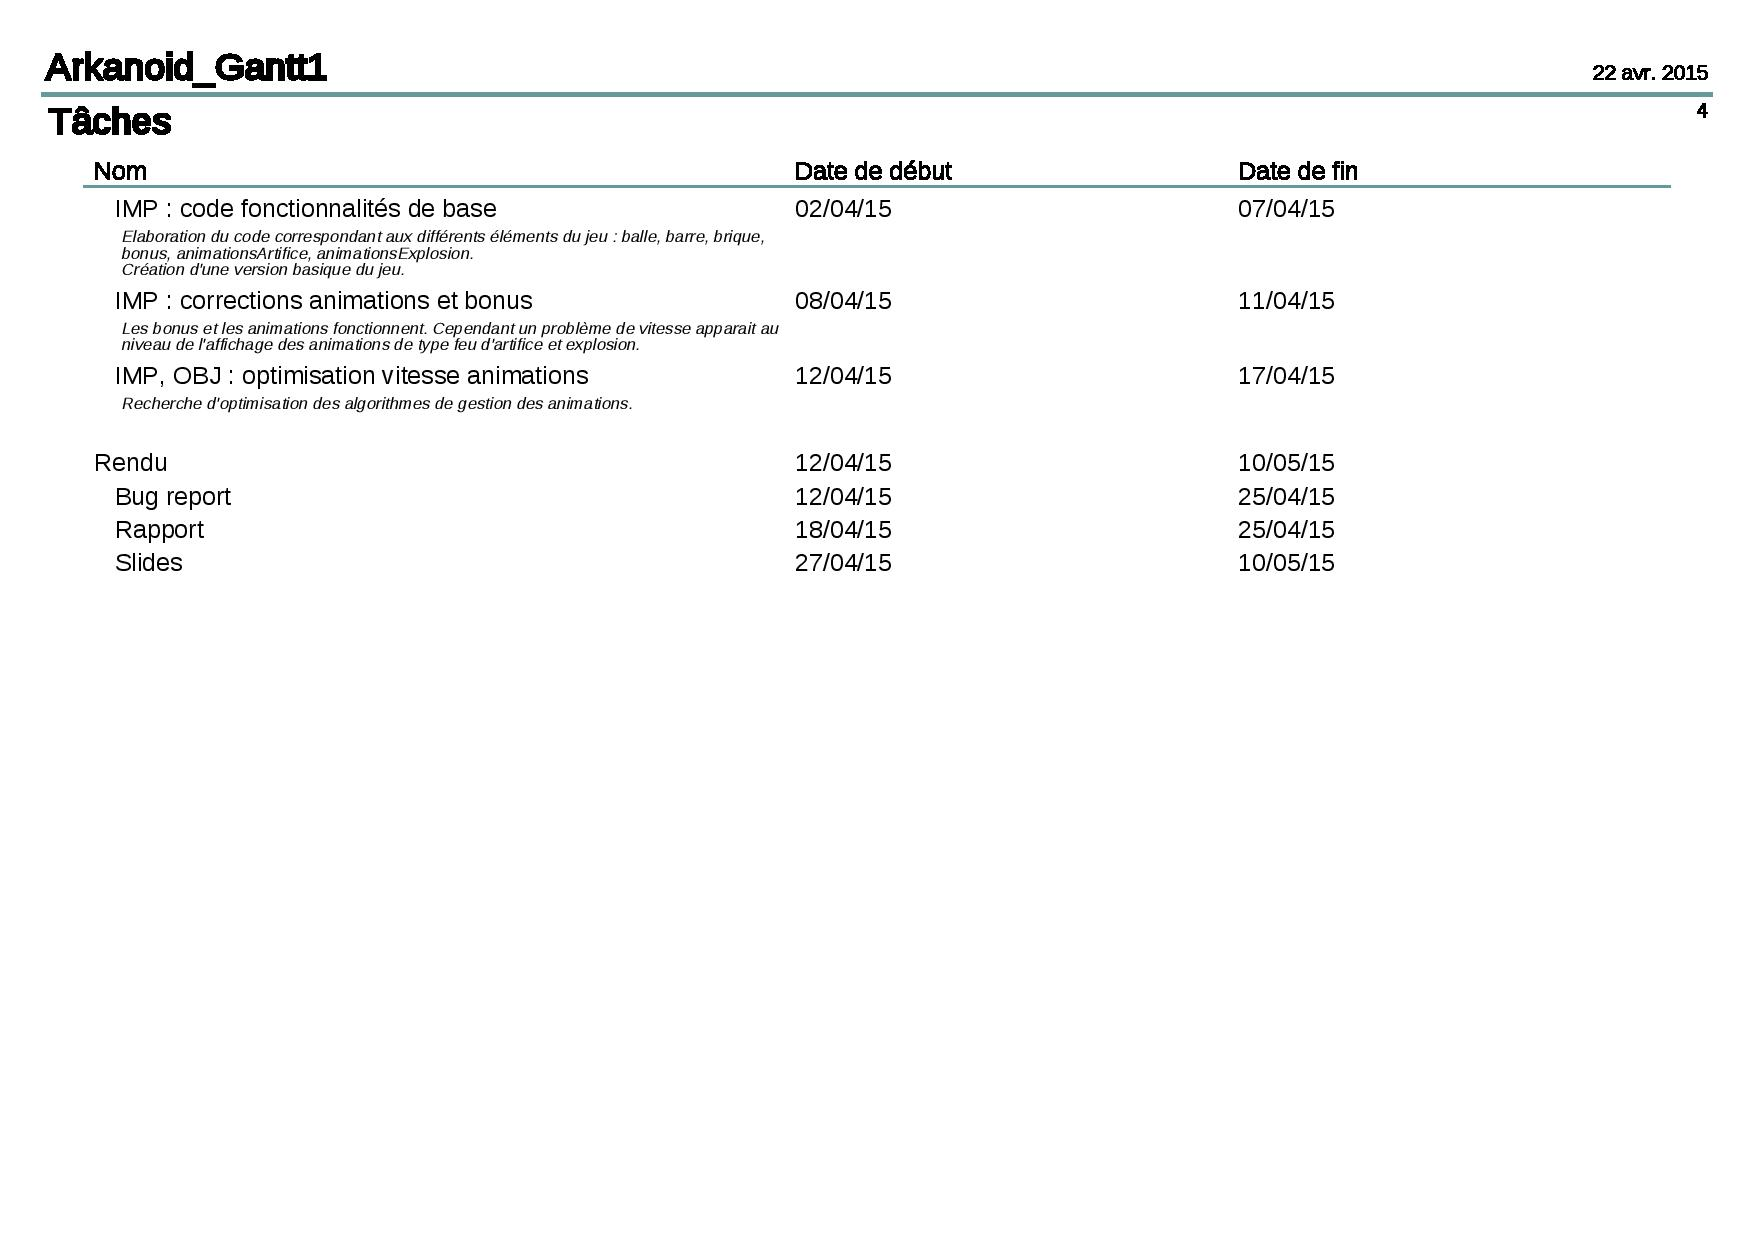
\includegraphics[width=1\textwidth]{img/WK3.jpg}\\
  \end{figure}
  
  \newpage
  \subsection{Diagramme de Gantt}
  	\begin{figure}[h!]
      \caption{Diagramme de Gantt}
      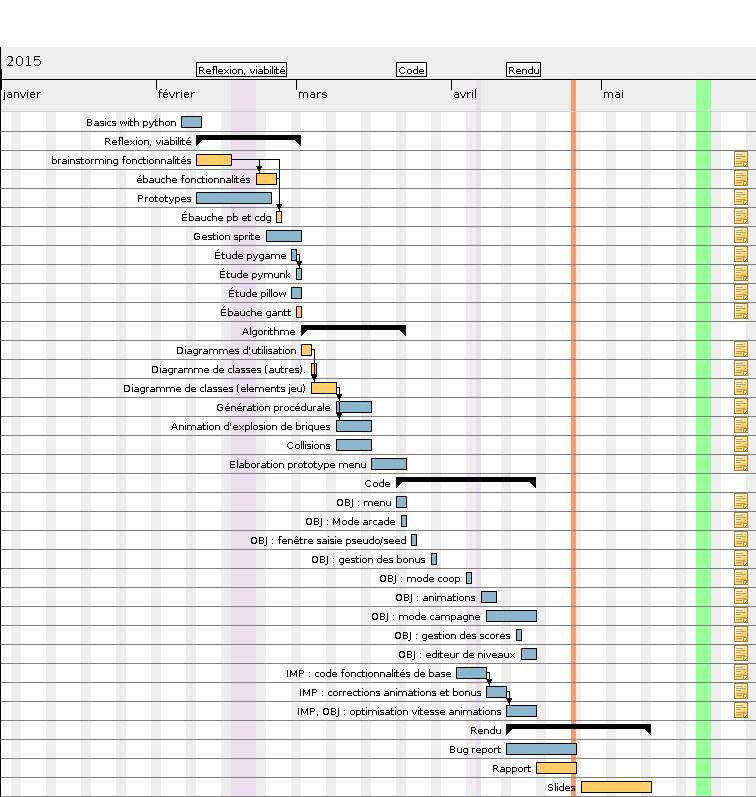
\includegraphics[width=1.1\textwidth]{img/gantt.jpg}\\[2em]
    \end{figure}
  
  \newpage
  \subsection{collision.py : fonction procgen}
  	\begin{minipage}{1\textwidth}
  	  \lstinputlisting[caption=fonction procgen, language=Python]{rsc/procgen.py}\nopagebreak
  	\end{minipage}
  	
  	Voir la section developpement technique pour de plus amples explications sur la stratégie adoptée. la fonction {\bf \em seed} (l 24), du module {\bf \em random}, permet de paramétrer la génération de nombre pseudo-aléatoire sur une graine. {\bf \em noise} correspond à une matrice de chiffre, correspondant aux pv des futurs briques. La fonction {\bf \em enlever} vient redéfinir certain de ces chiffres à 0. La variable {\em TESTING} n'est vrai que si et seulement si le programme est en test unitaire.

  \newpage
  \subsection{Working tree}
    \begin{figure}[hb!]
  	  \caption{Capture d'écran du working tree de git}
  	  \centering
  	  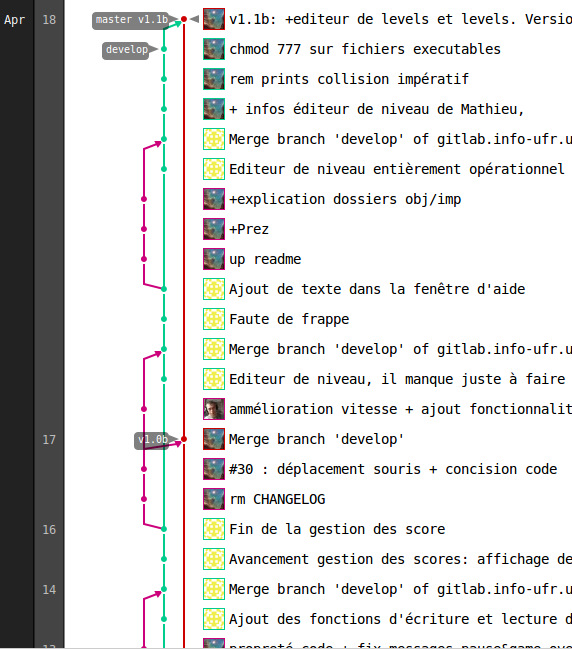
\includegraphics[width=1.1\textwidth]{img/workingtree.jpg}\\[2em]
  	\end{figure}
  	On pourra au passage noter notre gestion du système de tag
  
  \newpage
  \subsection{Issues}
  	\begin{figure}[hb!]
   	  \caption{Capture d'écran des issues de git}
  	  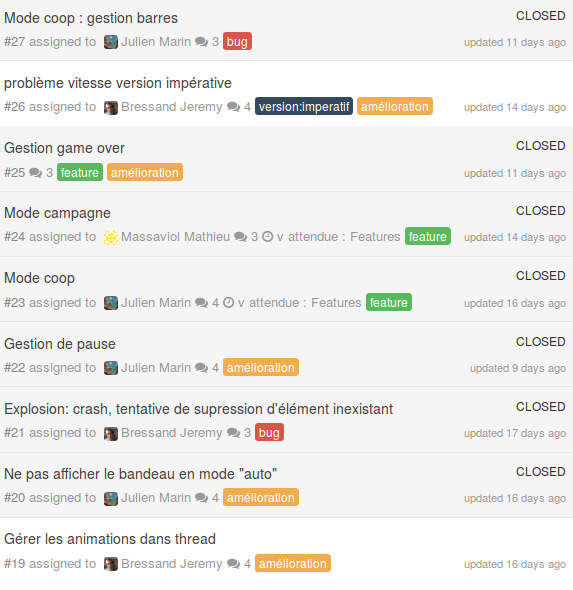
\includegraphics[width=1.1\textwidth]{img/issues.jpg}\\[2em]
  	\end{figure}
  
  \newpage
  \subsection{Bug report}
    \begin{enumerate}
       % Partie Jerem ...
       \item[\bf $\times$] Lorsque la balle est coincée entre la barre et le mur et que la barre fait pression contre la balle, la balle est éjectée de l'aire de jeu.

      \item[\checkmark] Bug variation vitesse balle lors de la collision avec la barre : Lors de la collision entre une balle et une barre, la vitesse de la balle varie de manière innatendue.
        \begin{itemize}
            \item[$\rightarrow$] Le problème a été résolu par un passage par angle, permettant d'obtenir une norme constante -- dans notre cas, une vitesse.
        \end{itemize}

      \item[\bf $\times$] Lorsque la barre reçoit le bonus d'agrandissement et qu'elle se trouve près du mur, elle se retrouve coincée dans celui ci.

      \item[\checkmark] Des briques supposées avoir un nombre de point de vie différents sont détruites au bout du même nombre de coups.
        \begin{itemize}
            \item[$\rightarrow$] Le problème était dû à une comparaison "inférieure" au lieu de "inférieure ou égale".
        \end{itemize}

      \item[\bf $\times$] Lors de collision balle/barre, il arrive dans de rares cas que la balle ne rebondisse pas de manière logique : elle inverse sa direction horizontale au lieu de sa direction verticale, ou inversement. 
       % Partie Marin
      \item[\checkmark] Crash du jeu lorsqu'une brique explosive en détruit plusieurs autres.
        \begin{itemize}
            \item[$\rightarrow$] Le programme éssayait de supprimer des briques déjà supprimées. Nous avons donc effectué la suppression avec la gestion de l'explosion.
        \end{itemize}
      \item[\checkmark] En mode coopératif, la position des barres des deux joueurs s'inversent, et une barre n'est pas supprimée - laissant une troisième barre "fantôme".
      \begin{itemize}
        \item[$\rightarrow$] Rien de conceptuel, nous avions simplement codé le mode coop trop rapidement.
      \end{itemize}

      \item[\checkmark] Vitesse anormale de la balle lorsqu'elle heurte un bord vertical d'une barre en mouvement.
      \begin{itemize}
        \item[$\rightarrow$] On ajoutait la vitesse de la barre à la balle, afin d'éviter qu'elles se retrouvent l'une dans l'autre. On a résolu le problème en plafonnant la vitesse horizontale de la balle à celle de la barre dans ce cas.
      \end{itemize}
      \item[\bf $\times$] Lorsque l'on commence une partie après en avoir finie une (ie être retourné au menu), le jeu commence en pause
      \item[\bf $\times$] En version imperative, le bonus d'ajout de balle créée une balle bien plus lente que les autres jusqu'à collision avec la barre.
    \end{enumerate}
  
